\chapter{Long-term trends in annual ground snow maxima}
\label{cha:time_trend}

% **************************** Define Graphics Path **************************
\ifpdf
    \graphicspath{{Chapter5/Figs/Raster/}{Chapter5/Figs/PDF/}{Chapter5/Figs/}}
\else
    \graphicspath{{Chapter5/Figs/Vector/}{Chapter5/Figs/}}
\fi

% **************************** Chapter Abstract ******************************
\leftskip=1cm
\noindent
\emph{The current structural design provisions are prevalently based on experience and on the assumption of stationary meteorological conditions. However, the observations of past decades and advanced climate models show that this assumption is debatable. Therefore, this chapter examines the historical long-term trends in ground snow load maxima and their effect on structural reliability. Annual maxima snow water equivalents are taken and univariate generalized extreme value distribution is adopted as a probabilistic model. Stationary and five non-stationary distributions are fitted to the observations utilizing the maximum likelihood method. Statistical and information theory based approaches are used to compare the models and to identify trends. Finally, reliability analyses are performed on a simple structure to explore the practical significance of the trends. The calculations show decreasing trends in annual maxima for most of the region. Although statistically significant changes are detected at many locations, the practical significance -- with respect to structural reliability -- is considerable only for a few, and the effect is favorable. The results indicate that contrary to the widespread practice in extreme event modeling, the exclusive use of statistical techniques on the analyzed extremes is insufficient to identify practically significant trends. This should be demonstrated using practically relevant examples, such as reliability of structures.}

\leftskip=0pt\rightskip=0pt

\mynote{it would be interesting to make a simple analysis regarding duration of snow covar, number of days with snow cover, maybe an annex}

%****************************************************************************************
%****************************************************************************************
\section{Problem statement and the state of the art}

The provisions of current structural standards are based on the assumption that the underlying natural phenomena -- generating the actions on structures, and determining their working environment -- are stationary. However, observations of the past decades and advanced meteorological analyses show that this assumption does not represent accurately the present, either the future world \citep{IPCC2012extremes, Milly2008, Herring2015}. Hence, the aim of this chapter is to analyze the long-term trends in snow events and their implications on structural reliability. The Carpathian Region is selected for the study and the database presented in Section \ref{sec:data_under_study} is used.

Previous studies indicate that there is a statistically significant time-trend in snow events for the region. \citet{Birsan2014} have analyzed historical observations from Romania and detected decrease in snowfall days (82\% of stations) with substantial decrease in snow depth (18\% of stations) and also in snow coverage (29\% of stations). 

\mynote{\citet{Pecho2009} found statistically significant decrease(increase?, poor quality study, should be included?) in five-day total precipitation and fresh snow cover depth for Slovakia.} 

To our knowledge the long-term trends in extreme snow loads, e.g. annual maxima, for the Carpathian Region have not been sufficiently analyzed yet. Moreover, we are not aware of any study quantitatively analyzing the effect of time-trends in snow loads on structural reliability.  Although \citet{Pecho2009} and \citet{Sadovsky2007} examined time-trends in snow precipitation for the Slovakian Alps, their study is insufficiently documented, which  makes it difficult to evaluate the merit and value of their work. From the available information it appears that their approach  is not able to answer the main questions of this chapter.
%, e.g. statistical significant changes are claimed; however, neither the applied test nor the significance level are documented. A similar study by  of the same region is better documented but besides the limited scope of the study it contains conceptual errors, e.g. it is undocumented how the authors used the Kolmogorov-Smirnov test (null and alternative hypotheses) although even without these details its use is incorrect since that requires completely specified distribution function to be compared with observations \citep{Lilliefors1967}. This criterion is certainly not met in the study, thus the use of Kolmogorov-Smirnov test is erroneous. Moreover, the authors base their conclusions on the outcome that all tests are passed. This is a misinterpretation of statistical null hypothesis tests. Note that even if the tests were conducted correctly, the conclusions should have been supported by additional analysis due to the limitations of null hypothesis significance testing \citep{Carver1993, Wagenmakers2008}.

An excellent study is available for the Swiss Alps where \citet{Marty2012} detected statistically significant negative, long-term trends in annual snow depth. However, their analysis is focused on statistical significance testing and on return values. Thus, although indicating interesting tendencies, the practical significance of their results, e.g. with respect to structural reliability cannot be judged. This is partially inevitable since practical significance differs by end-users. Therefore, in this chapter a more pragmatic approach is promoted in which after the statistical analysis the practical significance of the findings is examined. The main interest here is the impact of snow trends on structural reliability, particularly on the probability of structural failure. Only historical observations are considered but a worthwhile extension would be to incorporate the projections of global climate models. In a recent study \citet{Ogorman2014} showed that no considerable change is expected in the 20-year return period extreme snow events for the North American region up to the end of the 21st century, though the impact on structural reliability is inconclusive since that is governed by rarer events.

%****************************************************************************************
%****************************************************************************************
\section{Solution strategy}

Univariate generalized extreme value (GEV) distribution is selected as it is widely accepted in extreme value analysis \citep{Klein2009} and was successfully applied for modelling extreme precipitations \citep{Coles2003catastrophes}, temperatures \citep{Guttorp2011}\mynote{one ref is missing, ot Eriksson2013}, discharges \citep{Hao2015}, wind speeds \citep{Hundecha2008} and waves \citep{Caires2006}. Stationary and non-stationary models are compared based on how likely the data are generated by each model. The considered non-stationary distributions with time-dependent parameters are summarized in Table \ref{tab:nonstat_dist}. The shape parameter is constant in all presented models, this is explained by that models with shape parameter linearly varying in time yielded to considerably worse fit than the others and often lead to unrealistic fractiles. The adopted block length is one year, covering a whole winter season. Furthermore, to account for seasons without snow the cumulative distribution function of annual maxima is expressed as follows:
\begin{equation}
	P\left( {X < x} \right) = P\left( {{\mathrm{snowfall}}} \right) \cdot P\left( {X < x|{\mathrm{snowfall}}} \right)
\end{equation}
where the former event has Bernoulli, while the latter has GEV distribution.

Maximum likelihood method is selected for parameter estimation due to the large number of locations. According to \citet{Hosking1985} and \citet{Martins2000} the maximum likelihood method can lead to unstable parameter estimation for small sample size; however, it is deemed to be sufficient for this exploratory analysis. Bayesian approach might be used to overcome the issue of instability for further detailed studies.
\mynote{The method of moments is not suitable to handle non-stationary models, since the aggregated statistics (moments) do not contain information about the order of the observations, which is crucial to capture time-dependency (Section \ref{subsec:point estiamtes}).}

\begin{table}[htbp!]
\caption{Summary of the considered non-stationary GEV distributions.}
\centering
\label{tab:nonstat_dist}
\small
    \begin{tabular}{llll}
    \toprule
    Model ID  & Location par. ($\mu$) & Scale par. ($\sigma$) & Shape par. ($\xi$) \\ 
    \midrule
    \rowcolor{lightgrey} $\mu 1$  & $a_0 + a_1 \cdot t$  & constant  & constant \\
    $\mu 2$  & $b_0 + b_1 \cdot t+ b_2 \cdot t^2$  & constant   & constant \\
    \rowcolor{lightgrey} $\sigma 1$  & constant  & $d_0 + d_1 \cdot t$  & constant \\
    $\sigma 2$  & constant  & $e_0 + e_1 \cdot t+ e_2 \cdot t^2$  & constant \\
    \rowcolor{lightgrey} $\mu 1\sigma 1$ & $g_0 + g_1 \cdot t$  & $g_2 + g_3 \cdot t$ & constant   \\ 
    \bottomrule
    \end{tabular}
\end{table}

Likelihood ratio (LR) test and Akaike information criterion (AIC) are used to compare the stationary and non-stationary models. The former is a standard frequentist hypothesis test for comparing nested models \citep{Wilks1938}. The latter is an asymptotic information criterion that is based on the premise that the model with smallest information loss (Kullback-Leibler divergence) should be preferred \citep{Wit2012}. In the absence of the true model, the information loss cannot be calculated in absolute terms; however, the models can be compared and their relative ``strength'' can be expressed by the difference in AICs or by using Akaike weights (Eq.\ref{eq:Akaike_weight}). Herein the corrected form of Akaike information criterion (AICc, Eq.\ref{eq:AICc}) is applied that takes into account the effect of a finite sample size. The goodness-of-fit of the models is visually checked using Q–Q, P–P, and return-period–-return value plots \citep{Coles2001}. These plot types are defined in Annex~\ref{sec:prob_plots}. Additionally, at some locations the GEV model is compared to other commonly applied distributions for diagnostic purposes, i.e. Gumbel and three-parameter Lognormal. Due to the limitations of statistical significance testing \citep{Carver1993} the effect size, power of the test, and confidence intervals are also utilized to compare the models. The conclusions are based on the practical bearing of these models on structural reliability.

%****************************************************************************************
%****************************************************************************************
%\section{Results and discussion}

%****************************************************************************************
%\subsection{Historical observations 1962-2011}

%****************************************************************************************
%****************************************************************************************
\section{Stationary model}
Stationary GEV distribution is fitted to each of the 5895 grid points using the ML method; the corresponding shape parameters are plotted in Figure~\ref{fig:shape_map}. This map and all the others in the following are created using equidistant conic projection and linear interpolation. In Figure~\ref{fig:shape_map}, the areas bounded by black contours indicate Weibull distribution, it can be seen that the high mountainous areas have dominantly this upper bounded distribution type. Considerable part of the studied area has Fréchet distribution with relatively large shape parameter ($\xi > 0.2$), which is in conflict with the Gumbel assumption widely accepted in Europe \citep{Sanpaolesi1998}, EN 1991-1-3:2003 and ISO 4355:2013. Additional limitation of the Gumbel distribution is that it yields to artificially narrower confidence intervals than the Fréchet as its parameters span smaller space, see Chapter \ref{cha:stat_unc} and \citet{Coles2003catastrophes}.

\begin{figure}[htbp!]
	\centering    
	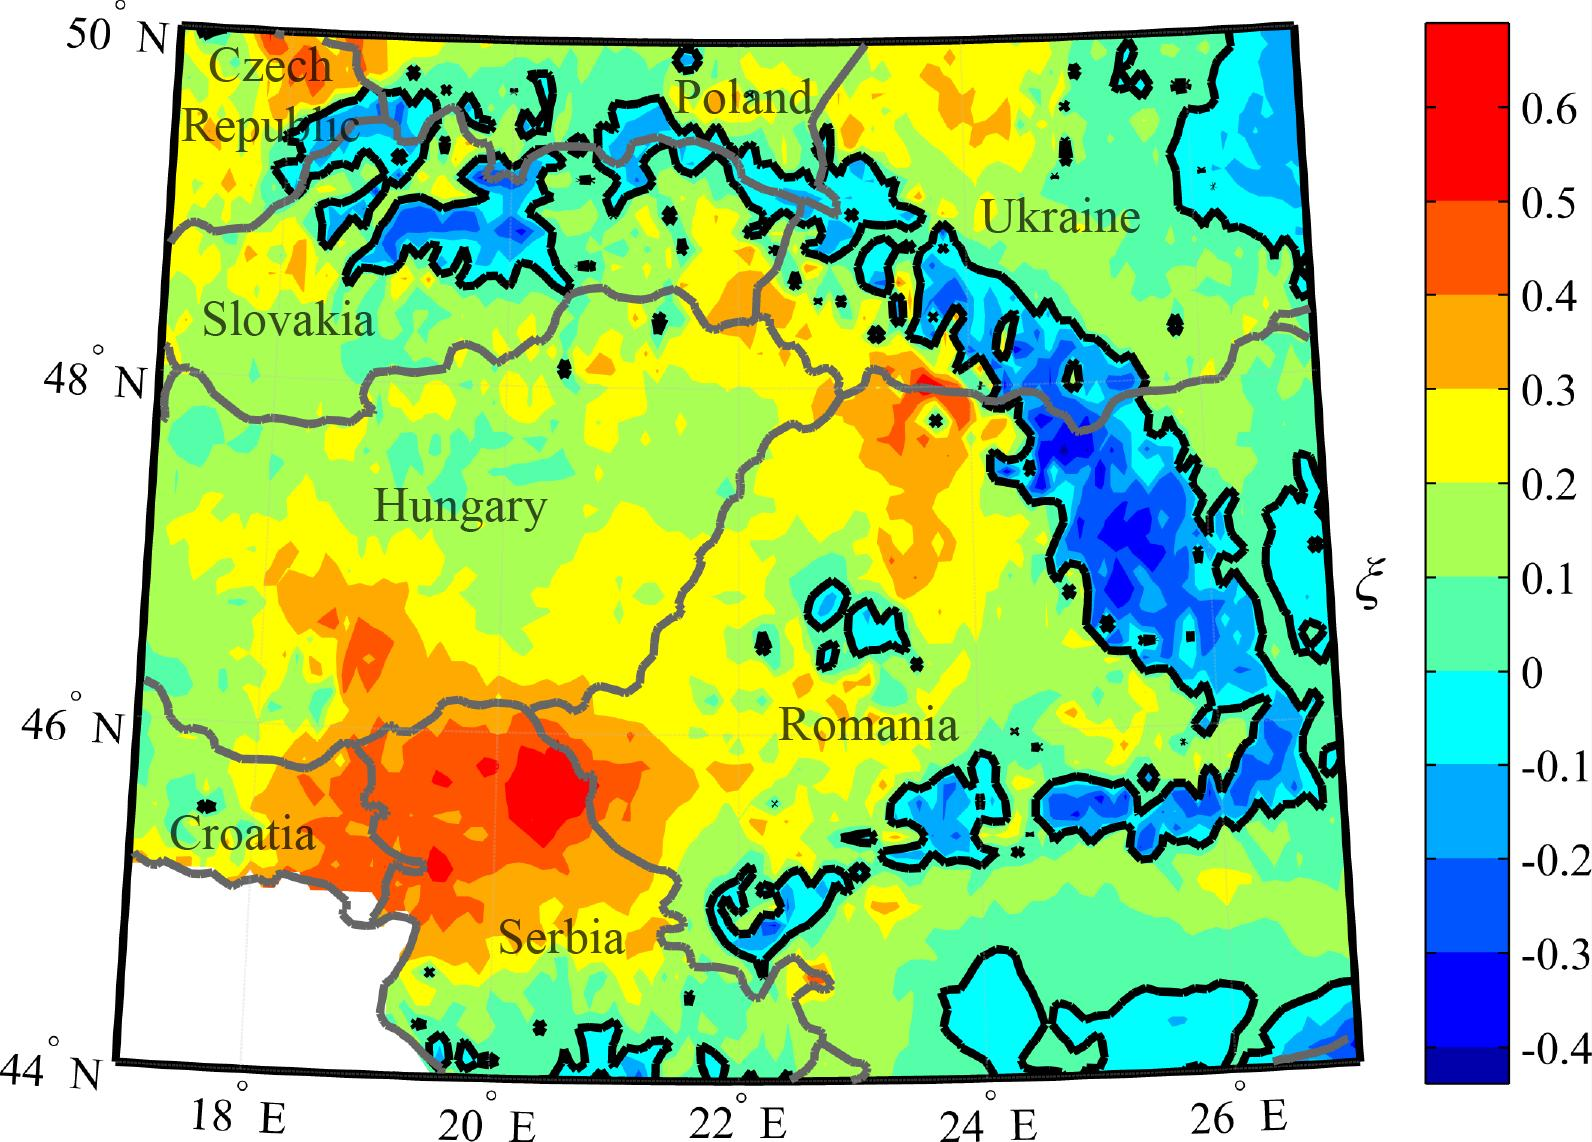
\includegraphics[width=0.5\textwidth]{stat_shape_parameter_map_crude_names.jpg}
	\caption{Shape parameter ($\xi$) of the fitted, stationary GEV distributions, the black contour surrounds the Weibull type.}
	\label{fig:shape_map}
\end{figure}

The unfavorable deviation from Gumbel distribution is the most pronounced in the northern part of Serbia. It is interesting that some locations exhibit shape parameter larger than 0.5, which means that the distribution has infinite variance. If this is deemed to be unrealistic, it might be avoided by adopting constraints in ML or by using Bayesian approaches with appropriate priors.

%****************************************************************************************
%****************************************************************************************
\section{Long-term trends, non-stationary models}
First, a straight line is fitted to the annual maxima (Figure~\ref{fig:trend_line}) at every grid point in the least-squares sense, while the snow-free years are discarded from the analysis. The associated slope parameters are illustrated in Figure~\ref{fig:trend_map}, where the negative values are referring to decreasing trends in time. At 97\% of the locations decreasing trend is identified, whereas a mild increase is observed in the northern part of the region -- Slovakia, the Czech Republic, and Poland. The small regions with strong, increasing trends next to decreasing ones (orange areas surrounded by dark blue ones) in Slovakia and Ukraine imply discrepancy in the database. Areas with the most pronounced decreasing trend are matching well with the Weibull regions with the exception of the southern part. Based on the linear trend the average change in annual maxima for the entire region during observation period is -42\%, compared to the 1962 level.

\begin{figure}[htbp!]
	\begin{subfigure}[b]{0.43\textwidth}    
		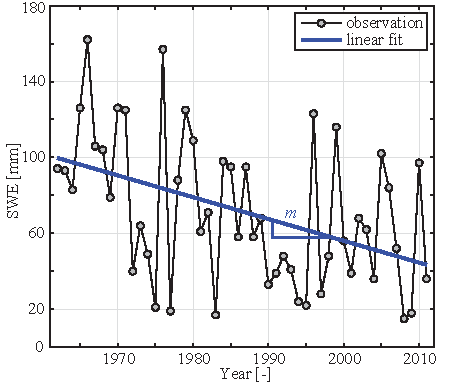
\includegraphics[width=\textwidth]{sample_time_trend.pdf}
		\caption{A representative location with decreasing trend.}
		\label{fig:trend_line}
	\end{subfigure}
	\hfill
	\begin{subfigure}[b]{0.52\textwidth}
		\includegraphics[width=\textwidth]{amax_timetrend_linreg_slope_paper.jpg}
		\caption{Map of the linear trend line’s slope parameter $m$ in mm/year.}
		\label{fig:trend_map}
	\end{subfigure}
	\caption{Fitting linear line to the annual maxima ground snow loads.}
\end{figure}

A more involved, LR and Akaike weight based comparisons of the stationary and five non-stationary GEV distributions show that the models with time-variant location parameters fit better the observations than those with time-variant scale parameter. Comparison between the models with time-variant location parameter reveals that the $\mu 1$ model performs the best for most of the area. The LR and Akaike weight based results, comparing the $\mu 1$ and stationary models are presented in Figure~\ref{fig:LR_mu1} and \ref{fig:AW_mu1}. Albeit both figures are showing probabilities ($P$), their interpretation is substantially different. In case of the LR test it expresses the probability that if the null hypothesis is true (stationary model) the difference between the log-likelihoods is at least as large as the one observed. This probability is typically referred as the $p$-value, and Figure~\ref{fig:LR_mu1} is showing the complementer of it ($P = 1 - p$). On the other hand, the Akaike weights –- illustrated in Figure~\ref{fig:AW_mu1} -– express the probability that $\mu 1$ model is better than the stationary one in the Kullback-Leibler divergence sense. In respect of these probabilities, the selected threshold is 90\% in both cases. Locations above this value are marked with a dot and considered as statistically significant. The vast majority of the statistically significant trends identified by the LR test are decreasing (black dots), only two locations in the Czech Republic show significant increase (white dots in the upper left corner in Figure~\ref{fig:LR_mu1}). The Akaike weight based comparison shows solely decreasing trends. The LR test is identified much more locations with significant trend, although the probabilities are not directly comparable. In addition, 65\% of these locations are statistically significant even with 95\% threshold level as well. The trends might be explained by the diminishing number of snow days as a consequence of increasing mean global temperature.

\begin{figure}[htbp!]
	\begin{subfigure}[b]{0.49\textwidth}    
		\includegraphics[width=\textwidth]{LR_test_stat_m1_p0_90_crude.jpg}
		\caption{Likelihood ratio.}
		\label{fig:LR_mu1}
	\end{subfigure}
	\hfill
	\begin{subfigure}[b]{0.49\textwidth}
		\includegraphics[width=\textwidth]{A_weight_stat_m1_p0_90_crude.jpg}
		\caption{Akaike weight.}
		\label{fig:AW_mu1}
	\end{subfigure}
	\caption{Comparison of $\mu 1$ and stationary models, grid-points with $P > 0.90$ are marked with dots: black for decreasing and white for increasing trends.}
\end{figure}

A more pragmatic comparison of time-trends is presented in Figure~\ref{fig:char_nonstat}, where the 50-year return values for stationary and non-stationary $\mu 1$ models are compared. The 50-year return value is referred as characteristic value in structural engineering and serves as the basis of everyday design. All the selected locations, shown in Figure~\ref{fig:char_nonstat}, exhibit significant negative trend in AICc sense.

\begin{figure}[htbp!]
	\centering
	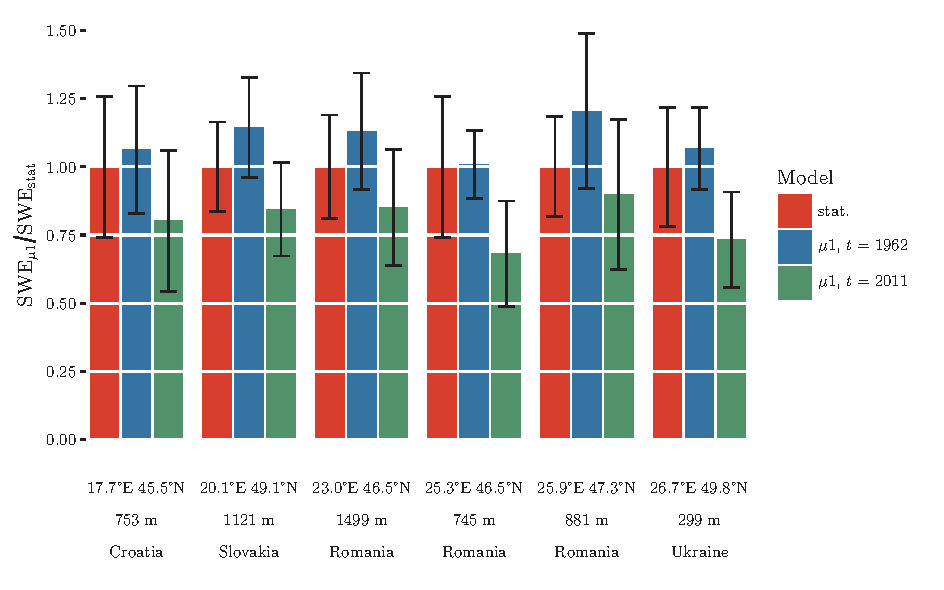
\includegraphics[width=1\textwidth]{char_values_stat_nonstat.pdf}
	\caption[]{Normalized 50-year return value SWE with 90\% confidence intervals (black) for selected locations that have significant negative trends as identified by Akaike weights \mynote{\footnotemark}.}
	\label{fig:char_nonstat}
\end{figure}
%\footnotetext{The countries are identified by ISO 3166-1 Alpha-3 codes.}

Figure~\ref{fig:char_nonstat} also shows that even for the locations where the AICc based criterion identified significant trends, in respect of 50-year return value with 90\% confidence interval, the difference is not always practically significant. The time-trend is deemed practically significant if the stationary estimate is outside of the non-stationary confidence interval. For the entire region, the average change characteristic values between 1962 and 2011 is $-10\%$, using the $\mu 1$ model and 1962 as reference. For locations with statistically significant trends the changes are $-19\%$ and $-26\%$ for LR test and Akaike weights respectively.

%****************************************************************************************
%****************************************************************************************
\section{Impact on structural reliability}

Although the focus of this chapter is the statistical characterization of snow loads and identification of trends in annual maxima, the key question from an engineering point \mynote{do not break here!!} of view is the effect of the changes on structural reliability and the adequacy of current provisions. The simple statistical, information theory (LR, AICc), and representative fractile based comparisons cannot answer this question, since the failure probability of a structure is dominantly determined by the tail of the distribution functions, well above or below the characteristic value. Thus, a simple, illustrative example is selected to explore this question. The related limit state function and the properties of the random variables are given in Eq.~\ref{eq:time_trend_gfun} and in Table~\ref{tab:time_trend_probmod}, respectively. For simplicity, the distribution functions of annual snow maxima are used and annual failure probabilities are calculated. Exceptional snow loads and accidental load combinations are not covered in the analysis.
\begin{equation}
\label{eq:time_trend_gfun}
	g = R - \left( {G + \mu  \cdot S } \right)
\end{equation}


\begin{table}[htbp!]
\caption{Summary of the considered non-stationary distributions.}
\centering
\label{tab:time_trend_probmod}
\small
	\begin{threeparttable}
    \begin{tabular}{lllll}
    \toprule
    Variable  & Distribution & Mean & CV & Reference \\
    \midrule
    \rowcolor{lightgrey} Resistance, $R$  & Lognormal & 1000/350\tnote{*} & 0.12  & \cite{JCSS_resi}  \\
    Ground snow, $S$ & GEV & \tnote{\textdagger} & \tnote{\textdagger}  & --  \\
    \rowcolor{lightgrey} Ground to roof conversion factor, $\mu$  & Lognormal & 0.75 & 0.15  & \cite{JCSS_load}  \\
    Permanent action, $G$  & Normal & 50 & 0.10  & \cite{JCSS_load}  \\
    \bottomrule
    \end{tabular}
    \begin{tablenotes}
    	\item[*] 1000 for the Hungarian, and 350 for the Ukrainian locations to achieve realistic and comparable reliability level.
	    \item[\textdagger] varies according to the selected model.  
   	\end{tablenotes}
   	\end{threeparttable}
\end{table}

Reliability analyses are performed for two representative locations using standard, first order reliability analysis (FORM). The first one is the Ukrainian location presented in Figure~\ref{fig:char_nonstat}. It has small, scattered settlements and it represents the significant negative trend even in respect of 50-year return values. The second is the fifth most populous city in Hungary (Pécs), it is identified by the LR test with statistically significant negative trend. It represents the moderate negative trend, which reflects well the majority of the region. These two locations are referred hereinafter as Ukrainian and Hungarian. Reliability is analyzed considering a reference period of one year. The location parameter is obtained from the non-stationary model for each of the selected years: 1962, 2011 and 2062. The delta method is used to construct approximate confidence intervals for these indices, and the results are summarized in Figure~\ref{fig:beta_nonstat}.

\begin{figure}[htbp!]
	\centering
	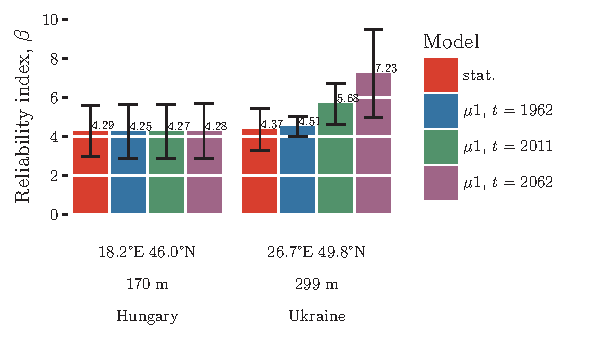
\includegraphics[width=0.7\textwidth]{beta_values_stat_nonstat.pdf}
	\caption{Reliability indices with 75\% confidence intervals (black) from ground snow parameter estimation uncertainty.}
	\label{fig:beta_nonstat}
\end{figure}

From Figure~\ref{fig:beta_nonstat} it is clear that the moderate decreasing trend has almost no effect on structural reliability, it is dwarfed by the parameter estimation uncertainty. For the Ukrainian location the increase in reliability level is practically significant, although the uncertainty is large here as well. From safety point of view, the change is clearly favorable, and whether the current provisions will provide economical design for these locations in the future is a different issue. The most important factor in the difference of the results for the Hungarian and Ukrainian locations is that the former has Fréchet while the latter has Weibull distribution.
The extrapolation of the non-stationary model to 2062 should be handled with care, it is provided only for illustrative purposes. It introduces additional uncertainty for non-stationary models as illustrated for the Ukrainian location in Figure~\ref{fig:extrap_nonstat}. This should be reduced by use of physical models or further explanations. 

\begin{figure}[htbp!]
	\centering
	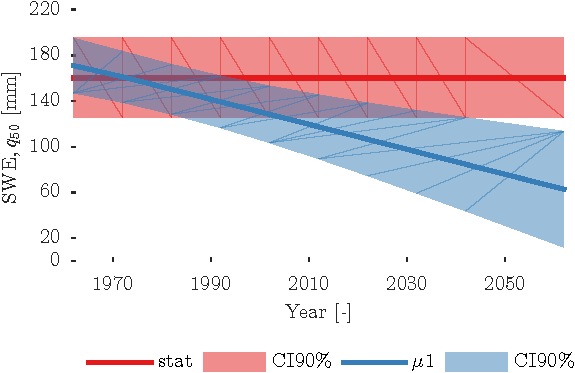
\includegraphics[width=0.7\textwidth]{stat_nonstat_conf_int_time_02.pdf}
	\caption{Ukrainian location, 50-year return value SWE ($q_{50}$) with 90\% confidence bands (CI90\%) for stationary (stat) and $\mu 1$ models.}
	\label{fig:extrap_nonstat}
\end{figure}

%***************************************************************************************
\subsection{Application example: Turbine hall of Paks Nucelar Power Plant}
\label{sec:turbine_trend}

Non-stationary extreme value analyses of annual ground snow maxima are conducted for the site of the turbine hall of Paks Nuclear Power Plant. The structure is introduced in Annex~\ref{sec:paks}, here only the essential details, which are required to interpret the results, are provided. Table~\ref{tab:nonstat_fit_paks} summarizes the Akaike weights and some representative fractiles for the selected models; the parameters are estimated using maximum likelihood method. The Akaike weights favor the stationary model, while the second best model is the one with linearly varying location parameter ($\mu1$). The fractiles of non-stationary models show small decrease in time.

The stationary and $\mu1$ models are used to calculate the annual reliability index of the structure in three distinct years (1962, 2011, and 2062). Furthermore, the parameter estimation uncertainty of ground snow load model is propagated to reliability index by using the delta method. The results are presented in Table~\ref{tab:nonstat_beta_paks}, from which it is salient that parameter estimation uncertainty dominates over the time-trend caused change in reliability index.

\begin{table}[htbp!]
\caption{Akaike weights and representative fractiles of the fitted stationary and non-stationary GEV distributions for the site of Paks Nuclear Power Plant. Fractiles are given for the years of 1962 and 2011.}
\centering
\label{tab:nonstat_fit_paks}
\small
	\begin{threeparttable}
	    \begin{tabular}{llllll}
	    \toprule
	    \multirow{2}{*}{Model ID} & \multirow{2}{*}{$w$\tnote{*}} & \multicolumn{2}{l}{$q_{50}$ [kN/m$^2$]} & \multicolumn{2}{l}{$q_{1000}$ [kN/m$^2$]} \\
	     &  & 1962  & 2011 & 1962 & 2011 \\ 
	    \midrule
	    \rowcolor{lightgrey} stat.       & 0.439 & 1.53 & 1.53 & 4.83 & 4.83 \\
	    $\mu 1$                          & 0.190 & 1.55 & 1.49 & 4.82 & 4.76 \\
	    \rowcolor{lightgrey} $\mu 2$     & 0.092 & 1.57 & 1.50 & 4.64 & 4.56 \\
	    $\sigma 1$                       & 0.139 & 1.56 & 1.41 & 4.74 & 4.25 \\
	    \rowcolor{lightgrey} $\sigma 2$  & 0.054 & 1.75 & 1.53 & 4.99 & 4.29 \\
	    $\mu 1\sigma 1$                  & 0.085 & 1.80 & 1.11 & 5.38 & 3.35 \\
	    \bottomrule
	    \end{tabular}
    \begin{tablenotes}
        \item[*] Akaike weight.
    \end{tablenotes}
    \end{threeparttable}
\end{table}

\begin{table}[htbp!]
\caption{Annual reliability indices for the turbine hall considering stationary and non-stationary GEV distributed ground snow maxima. Reliability indices are accompanied by 90\% confidence intervals and they are given for the years of 1962, 2011 and 2062.}
\centering
\label{tab:nonstat_beta_paks}
\small
	\begin{threeparttable}
	    \begin{tabular}{llll}
	    \toprule
	    \multirow{2}{*}{Model ID} & \multicolumn{3}{c}{$\beta$\tnote{*}} \\
	     &  1962  & 2011 & 2062 \\ 
	    \midrule
	    \rowcolor{lightgrey} stat.  & 3.37 (2.35,4.41) & 3.37 (2.35,4.41) & 3.37 (2.35,4.41)  \\
	    $\mu 1$                     & 3.38 (2.33,4.43) & 3.39 (2.33,4.45) & 3.40 (2.33,4.46)  \\
	    \bottomrule
	    \end{tabular}
    \begin{tablenotes}
        \item[*] Maximum likelihood point estimate of annual reliability index with 90\% confidence interval in brackets.
    \end{tablenotes}
    \end{threeparttable}
\end{table}


%****************************************************************************************
%******************************************************************************************
\section{Discussion}
The results are dependent on the number of observations and on the reference period used in the reliability analyses. More data would yield to narrower confidence intervals and allow sharper/stronger conclusions, while an extended reference period would level out the differences in annual failure probabilities.

The adopted, practical-significance oriented approach could be applied for other issues as well and not restricted to snow extremes and structural reliability. A limitation of this study is that only GEV distributions are considered. This can have an important effect on the failure probability, since that is governed by the tail of the distribution, i.e. very rare, not even observed events. This is known in structural reliability as distribution arbitrariness \citep{Ditlevsen1994}. This effect could be investigated by more involved statistical techniques, but could be overcome only by using additional data or accurate physical models; these are rarely available.

In all analysis here, historical observations are used, though similar calculations are completed for the Carpathian Region considering climate projection until the end of the 21st century. The preliminary results indicate decreasing trend in ground snow load and negligible effect on structural reliability for some selected locations \citep{Kaman2014}. However, it requires further research to decide whether the results of global circulation models can reasonably predict such extremes that needed in structural reliability analyses. 

In spite of limitations, it is believed that the present analysis provides an interesting insight and considering the current state of knowledge in structural engineering it can support decision-making process.



%****************************************************************************************
%\section{Extension to other random variables}


\section{Summary and conclusions}

The following main conclusions are drawn from the statistical and information theory based time-trend analysis of annual ground snow maxima:
\begin{itemize}
	\item Based on the shape parameter of Generalized extreme value distribution, for the majority of lowland and highland locations Fréchet distribution seems to be appropriate, while Weibull distribution fits the data better for mountains.
	\item A decreasing trend in annual snow maxima is found for 97\% of the studied region.
	\item The LR test identified numerous locations with statistically significant ($p < 0.05$) decreasing trends. However, the power of the test on average is low, and the effect size compared to confidence intervals regarding the 50-year return value reveals substantial uncertainty.
	\item The likelihood ratio test and Akaike weights suggest that the trend in the annual maxima is better captured by allowing trend in the location parameter than in the scale parameter.
	\item The reliability analyses show that the practical significance of time trends is not implied by the statistical significance. This is largely due to the substantial uncertainty in the parameter estimation, dominating structural reliability.
	\item The reliability analyses indicate that for most locations in the region that are characterized by 
	Fréchet distribution the negative trend in annual snow maxima has a minor effect on structural reliability, the uncertainty in parameter estimation is governing. Moreover, it is deemed unjustified to extrapolate trends based on about 50 years to thousands of years, which represent a relevant return periods for the ultimate limit states.
	\item For locations with a strongly decreasing trend and Weibull distribution, the effect of the trend on structural reliability is practically significant, although it is favorable. 
\end{itemize}

